\documentclass[a4paper,10pt]{scrartcl}
\usepackage[pdftex]{graphicx}
\DeclareGraphicsExtensions{.pdf,.png,.jpg}
\RequirePackage[hyperindex]{hyperref}
\usepackage{amssymb}

\newcommand\cI{{\cal I}}
\newcommand\cT{{\cal T}}
\newcommand\cA{{\cal A}}
\newcommand\cK{{\cal K}}
\newcommand\cC{{\cal C}}
\newcommand\cL{{\cal L}}
\newcommand\fluffy{{\mathit{fluffy}}}

\newenvironment{example}{}{}
\newenvironment{definition}{}{}

\begin{document}
\title{TRILL Manual}

\subtitle{SWI-Prolog Version}

\author{Riccardo Zese\\
riccardo.zese@unife.it}

\maketitle


\section{Introduction}


TRILL (``Tableau Reasoner for descrIption Logics in Prolog'', \cite{ZesBelRig16-AMAI-IJ,Zese17-SSW-BK}) implements a tableau algorithm in
Prolog to compute the set of all the explanations of a query. 
TRILL also contains TRILL$^P$ (``TRILL powered by Pinpointing formulas''), which is able to compute a Boolean formula representing the set of explanations for a query, and 
TORNADO (``Trill powered by pinpOinting foRmula and biNAry DecisiOn diagrams'') which represent the pinpointing formula directly as a binary decision diagram, simplifying the management of the formula.
After generating the explanations, 
TRILL can computes the probability of the query. The management of the tableau rules' non-determinism is delegated to the Prolog language.

TRILL is available in two versions, one for Yap Prolog and one for SWI-Prolog. They differ slightly in the features offered.
The Yap version differs principally in the absence of the translation module form OWL/RDF to TRILL syntax and in a different management of the explanations in TRILL$^P$.

\section{Installation}
TRILL is distributed as a \href{http://www.swi-prolog.org/pack/list?p=trill}{pack} of \href{http://www.swi-prolog.org/}{SWI-Prolog}. To install it, use
\begin{verbatim}
?- pack_install(trill).
\end{verbatim}
Moreover, in order to make sure you have a foreign library that matches your architecture, run
\begin{verbatim}
?- pack_rebuild(trill). 
\end{verbatim}


\section{Syntax}
\label{syn}
\texttt{cplint} permits the definition of discrete probability distributions and continuous probaility
densities.
\subsection{Discrete Probability Distributions}
\label{discrete}
LPAD and CP-logic programs consist of a set of annotated disjunctive clauses.
Disjunction in the head is represented with a semicolon and atoms in the head are separated from probabilities by a colon. For the rest, the usual syntax of Prolog is used.
A general CP-logic clause has the form
\begin{verbatim}
h1:p1 ; ... ; hn:pn :- Body.
\end{verbatim}
where \verb|Body| is a conjunction of goals as in Prolog.
 No parentheses are necessary. The \texttt{pi} are numeric expressions. It is up to the user to ensure that the numeric expressions are legal, i.e. that they sum up to less than one.

If the clause has an empty body, it can be represented like this
\begin{verbatim}
h1:p1 ; ... ; hn:pn.
\end{verbatim}
If the clause has a single head with probability 1, the annotation can be omitted and the clause takes the form of a normal prolog clause, i.e. 
\begin{verbatim}
h1 :- Body.
\end{verbatim}
stands for 
\begin{verbatim}
h1:1 :- Body.
\end{verbatim}
The coin example of  \cite{VenVer04-ICLP04-IC} is represented as (file \href{http://cplint.eu/example/inference/coin.pl}{\texttt{coin.pl}})
\begin{verbatim}
heads(Coin):1/2 ; tails(Coin):1/2 :- 
  toss(Coin),\+biased(Coin).

heads(Coin):0.6 ; tails(Coin):0.4 :- 
  toss(Coin),biased(Coin).

fair(Coin):0.9 ; biased(Coin):0.1.

toss(coin).
\end{verbatim}
The first clause states that if we toss a coin that is not biased it has equal probability of landing heads and tails. The second states that if the coin is biased it has a slightly higher probability of landing heads. The third states that the coin is fair with probability 0.9 and biased with probability 0.1 and the last clause states that we toss a coin with certainty.

Moreover, the bodies of rules may contain built-in predicates, predicates
from the libraries \verb|lists|, \verb|apply| and \verb|clpr/nf_r|
plus the predicate
\begin{verbatim}
average/2
\end{verbatim}
that, given a list of numbers, computes its arithmetic mean.

The body of rules may also contain the predicate \verb|prob/2| that computes the
probability of an atom, thus allowing nested probability computations.
For example (\href{http://cplint.eu/example/inference/meta.pl}{\texttt{meta.pl}})
\begin{verbatim}
a:0.2:-
  prob(b,P),
  P>0.2.
\end{verbatim}
is a valid rule.

Moreover, the probabilistic annotations can be variables, as in 
(\href{http://cplint.eu/example/inference/flexprob.pl}{\texttt{flexprob.pl}}))
\begin{verbatim}
red(Prob):Prob.

draw_red(R, G):-
  Prob is R/(R + G),
  red(Prob).
\end{verbatim}
Variables in probabilistic annotations must be ground when resolution reaches the end of the body, 
otherwise an exception is raised.

Alternative ways of specifying probability distribution include
\begin{verbatim}
A:discrete(Var,D):-Body.
\end{verbatim}
or
\begin{verbatim}
A:finite(Var,D):-Body.
\end{verbatim}
where \verb|A| is an atom containg variable \verb|Var| and \verb|D|
is a list of couples \verb|Value:Prob| assigning probability \verb|Prob|
to \verb|Value|. 
Moreover, you can use
\begin{verbatim}
A:uniform(Var,D):-Body.
\end{verbatim}
where \verb|A| is an atom containg variable \verb|Var| and \verb|D|
is a list of values each taking the same probability (1 over the length
of \verb|D|).
\subsubsection{ProbLog Syntax}
You can also use ProbLog \cite{DBLP:conf/ijcai/RaedtKT07} syntax, so a general clause takes the form
\begin{verbatim}
p1::h1 ; ... ; pn::hn :- Body
\end{verbatim}
where the \texttt{pi} are numeric expressions. 

\subsubsection{PRISM Syntax}
You can also use PRISM \cite{DBLP:conf/ijcai/SatoK97} syntax, so a program is composed of
a set of regular Prolog rules whose body may contain calls to the \verb|msw/2| predicate (multi-ary 
switch). A call \verb|msw(term,value)| means that a random variable associated to \verb|term|
assumes value \verb|value|. The admissible values  for a discrete random variable are 
specified using facts for the \verb|values/2| predicate of the form
\begin{verbatim}
values(T,L).
\end{verbatim}
where \verb|T| is a term (possibly containing variables) and \verb|L| is a list of values.
The distribution over values is specified using directives for \verb|set_sw/2| of the form
\begin{verbatim}
:- set_sw(T,LP).
\end{verbatim}
where \verb|T| is a term (possibly containing variables) and \verb|LP| is a list of
probability values.
Remember that in PRISM each call to \verb|msw/2| refers to a different random
variable, i.e., no memoing is performed, differently from the case of LPAD/CP-Logic/ProbLog.

For example, the coin example above in PRISM syntax becomes
(\href{http://cplint.eu/example/inference/coinmsw.pl}{\texttt{coinmsw.pl}})
\begin{verbatim}
values(throw(_),[heads,tails]).
:- set_sw(throw(fair),[0.5,0.5]).
:- set_sw(throw(biased),[0.6,0.4]).
values(fairness,[fair,biased]).
:- set_sw(fairness,[0.9,0.1]).
res(Coin,R):- toss(Coin),fairness(Coin,Fairness),msw(throw(Fairness),R).
fairness(_Coin,Fairness) :- msw(fairness,Fairness).
toss(coin).
\end{verbatim}
\subsection{Continuous Probability Densities}
\label{cont}

\verb|cplint| handles continuous random variables as well with its
sampling inference module.
To specify a probability density on an argument \verb|Var| of an atom
\verb|A| you can used rules of the form
\begin{verbatim}
A:Density:- Body
\end{verbatim}
where \verb|Density| is a special atom identifying a probability  density on variable \verb|Var| and \verb|Body| (optional) is a regular clause body.
Allowed \verb|Density| atoms are
\begin{itemize}
\item \verb|uniform(Var,L,U)|: \verb|Var| is uniformly distributed in $[L,U]$
\item \verb|gaussian(Var,Mean,Variance)|: \verb|Var| follows a Gaussian distribution with mean \verb|Mean| and variance \verb|Variance|. The distribution can be multivariate if \verb|Mean| 
is a list and \verb|Variance| a list of lists representing the mean vector and the covariance matrix. In this case the values of \verb|Var| are lists of real values with the same length as
that of \verb|Mean|
\item \verb|dirichlet(Var,Par)|: \verb|Var| is a list of real
numbers following a Dirichlet distribution with $\alpha$ parameters specified
by the list \verb|Par|
\item \verb|gamma(Var,Shape,Scale)|  \verb|Var| follows a gamma distribution 
with shape parameter \verb|Shape| and scale parameter \verb|Scale|.
\item \verb|beta(Var,Alpha,Beta)|  \verb|Var| follows a beta distribution 
with parameters \verb|Alpha| and \verb|Beta|.
\item \verb|poisson(Var,Lambda)|  \verb|Var| follows a Poisson distribution 
with parameter \verb|Lambda|.
\item \verb|binomial(Var,N,P)|  \verb|Var| follows a binomial distribution 
with parameters \verb|N| and \verb|P|.
\item \verb|geometric(Var,P)|  \verb|Var| follows a geometric distribution 
with parameter \verb|P|.
\end{itemize}
For example
\begin{verbatim}
g(X): gaussian(X,0, 1).
\end{verbatim}
states that argument \verb|X| of \verb|g(X)| follows a Gaussian 
distribution with mean 0 and variance 1, while
\begin{verbatim}
g(X): gaussian(X,[0,0], [[1,0],[0,1]]).
\end{verbatim}
states that argument \verb|X| of \verb|g(X)| follows a Gaussian 
multivariate distribution with mean vector $[0,0]$ and covariance matrix
$$\left[\begin{array}{rr}
1&0\\
0&1
\end{array}\right]$$.



For example, \href{http://cplint.eu/example/inference/gaussian_mixture.pl}{\texttt{gaussian\_mixture.pl}} defines a mixture of two Gaussians:
\begin{verbatim}
heads:0.6;tails:0.4.
g(X): gaussian(X,0, 1).
h(X): gaussian(X,5, 2).
mix(X) :- heads, g(X).
mix(X) :- tails, h(X).
\end{verbatim}
The argument \verb|X| of
\verb|mix(X)| follows a distribution that is a mixture of two Gaussian,
one with mean 0 and variance 1 with probability 0.6 and one with 
mean 5 and variance 2 with probability 0.4.

The parameters of the distribution atoms can be taken from the probabilistic
atom, the example \href{http://cplint.eu/example/inference/gauss_mean_est.pl}{\texttt{gauss\_mean\_est.pl}}
\begin{verbatim}
val(I,X) :-
  mean(M),
  val(I,M,X).
mean(M): gaussian(M,1.0, 5.0).
val(_,M,X): gaussian(X,M, 2.0).
\end{verbatim}
states that for an index \verb|I| the continuous variable \verb|X| is 
sampled from a Gaussian whose variance is 2 and whose mean is sampled from a Gaussian with mean 1 and
variance 5.

Any operation is allowed on continuous random variables. The example below
(\href{http://cplint.eu/example/inference/kalman_filter.pl}{\texttt{kalman\_filter.pl}}) encodes a Kalman filter:
\begin{verbatim}
kf(N,O, T) :-
  init(S),
  kf_part(0, N, S,O,T).
kf_part(I, N, S,[V|RO], T) :-
  I < N,
  NextI is I+1,
  trans(S,I,NextS),
  emit(NextS,I,V),
  kf_part(NextI, N, NextS,RO, T).
kf_part(N, N, S, [],S).
trans(S,I,NextS) :-
  {NextS =:= E + S},
  trans_err(I,E).
emit(NextS,I,V) :-
  {NextS =:= V+X},
  obs_err(I,X).
init(S):gaussian(S,0,1).
trans_err(_,E):gaussian(E,0,2).
obs_err(_,E):gaussian(E,0,1).
\end{verbatim}
Continuous random variables are involved
in arithmetic expressions (in \verb|trans/3| and \verb|emit/3|). It
is often convenient, as in this case, to use CLP(R) constraints (by
including the directive \verb|:- use_module(library(clpr)).|) as 
in this way the expressions can be used in multiple directions and 
the same clauses can be used both to sample and to evaluate the weight the sample on the basis
of evidence,
otherwise different clauses have to be written.
In case random variables are not sufficiently instantiated to 
exploit expressions for inferring the values of other variables, 
inference will return an error.

\subsubsection{Distributional Clauses Syntax}
\label{dc}
You can also use the syntax of Distributional Clauses (DC) \cite{Nitti2016}.
Continuous random variables are represented in this case by term whose distribution can be specified with density atoms as in
\begin{verbatim}
T~Density' := Body.
\end{verbatim}
Here \verb|:=| replaces the implication symbol, \verb|T| is a term and \verb|Density'| is one of the density atoms above without the \verb|Var| argument, because \verb|T|
itself represents a random variables. In the body of clauses you can use the infix operator \verb|~=| to equate a term representing a random variable with a logical variable or
a constant as in \verb|T ~= X|. Internally \verb|cplint| transforms the terms representing random variables into atoms with an extra argument for holding the variable.
DC can be used to represent also discrete distributions using
\begin{verbatim}
T~uniform(L) := Body.
T~finite(D) := Body.
\end{verbatim} 
where \verb|L| is a list of values and \verb|D| is a list of couples \verb|P:V| with \verb|P| a probability and \verb|V| a value.
If \verb|Body| is empty, as in regular Prolog, the implication symbol \verb|:=| can be omitted.

The Indian GPA problem from \url{http://www.robots.ox.ac.uk/~fwood/anglican/examples/viewer/?worksheet=indian-gpa}in distributional clauses syntax  (\url{https://github.com/davidenitti/DC/blob/master/examples/indian-gpa.pl})
takes the form (\href{http://cplint.eu/example/inference/indian_gpadc.pl}{\texttt{indian\_gpadc.pl}}):
\begin{verbatim}
is_density_A:0.95;is_discrete_A:0.05.
% the probability distribution of GPA scores for American students is
% continuous with probability 0.95 and discrete with probability 0.05

agpa(A): beta(A,8,2) :- is_density_A.
% the GPA of American students follows a beta distribution if the
% distribution is continuous

american_gpa(G) : finite(G,[4.0:0.85,0.0:0.15]) :- is_discrete_A.
% the GPA of American students is 4.0 with probability 0.85 and 0.0
% with 
% probability 0.15 if the
% distribution is discrete
american_gpa(A):- agpa(A0), A is A0*4.0.
% the GPA of American students is obtained by rescaling the value of
% agpa
% to the (0.0,4.0) interval
is_density_I : 0.99; is_discrete_I:0.01.
% the probability distribution of GPA scores for Indian students is
% continuous with probability 0.99 and discrete with probability 
% 0.01
igpa(I): beta(I,5,5) :- is_density_I.
% the GPA of Indian students follows a beta distribution if the
% distribution is continuous
indian_gpa(I): finite(I,[0.0:0.1,10.0:0.9]):-  is_discrete_I.
% the GPA of Indian students is 10.0 with probability 0.9 and 0.0
% with
% probability 0.1 if the
% distribution is discrete
indian_gpa(I) :- igpa(I0), I is I0*10.0.
% the GPA of Indian students is obtained by rescaling the value 
% of igpa
% to the (0.0,4.0) interval
nation(N) : finite(N,[a:0.25,i:0.75]).
% the nation is America with probability 0.25 and India with 
% probability 0.75
student_gpa(G):- nation(a),american_gpa(G).
% the GPA of the student is given by american_gpa if the nation is 
% America
student_gpa(G) :- nation(i),indian_gpa(G).
% the GPA of the student is given by indian_gpa if the nation 
%is India
\end{verbatim}
See 

\section{Semantics}
\label{semantics}

The semantics of LPADs for the case of programs without functions symbols can be given
as follows. An LPAD defines a probability distribution over normal logic programs called
\emph{worlds}. A world is obtained from an LPAD by first grounding it, by 
selecting a single head atom for each ground clause and by including in the world
the clause with the selected head atom and the body.
The probability of a world is the product of the probabilities associated to the 
heads selected.
The probability of a ground atom (the query) is given by the sum of the probabilities
of the worlds where the query is true.

If the LPAD contains function symbols, the definition is more complex, see
\cite{DBLP:journals/ai/Poole97,DBLP:journals/jair/SatoK01,Rig15-PLP-IW}.

For the semantics of programs with continuous random variables, see \cite{TLP:8688161}
that defines the probability
space for $N$ continuous random variables by considering the Borel $\sigma$-algebra
over $\mathbb{R}^N$
and defines a Lebesgue measure on this set as the probability measure.
The probability space is lifted to cover the entire program using the least model semantics of constraint logic programs. Alternatively,
\cite{Nitti2016} defines the semantics of distributional clauses by resorting to
a stochastic $Tp$ operator.
\verb|cplint| allows more freedom than distributional clauses in the use of continuous random variables
in expressions, for example
\href{http://cplint.eu/e/kalman_filter.pl}{\texttt{kalman\_filter.pl}} would not be allowed by distributional clauses.

\section{Inference}
\label{inf}

TRILL systems can answer many different queries. To do so, it exploits an algorithm called \emph{tableau} algorithm, which is able to collect explanations. In the following you can find an example that shows how the tableau works. In section~\ref{sec:trillq} we will see how queries can be asked with TRILL systems.

Consider a simple knowledge base inspired by the film ``The Godfather'' containing the following axioms:
\begin{align}
&tom : Cat\\
&(donVito, tom) : hasPet\\
&Cat \sqsubseteq Pet\\
&\exists hasAnimal.Pet \sqsubseteq NatureLover\\
&NatureLover \sqsubseteq GoodPerson\\
&hasPet \sqsubseteq hasAnimal
\end{align}

The axioms are telling what is known about the domain: (1) Tom is an individual of the domain, and he is a Cat; (2) donVito (Vito Corleone) has tom as his pet; (3) all cats are also pets; (4) everyone having at least one animal which is a pet is a nature lover; (5) nature lovers are good people; and (6) if one has a pet, she/he also has an animal.

This KB can be defined by the following TRILL syntax axioms:
\begin{verbatim}
classAssertion(cat, tom).
propertyAssertion(hasPet, donVito, tom).
subClassOf(cat, pet).
subClassOf(someValuesFrom(hasAnimal, pet), natureLover).
subClassOf(natureLover,goodPerson).
subPropertyOf(hasPet,hasAnimal).
\end{verbatim}

The first two axioms are assertional axioms (hence they constitute the ABox), the other four axioms define the TBox. Axiom 1 is called class assertion, 2 is called property assertion, 3,4,5 are called class subsumption axioms, and axiom 6 is called property subsumption axiom.

To check, for example, whether don Vito Corleone is a good person, the tableau algorithm builds a graph, called the \emph{tableau}. The initial tableau contains information from the ABox plus the negation of the query, as depicted in Figure\ref{fig:tab1}. This last axiom is added since the underlying proof mechanism uses refutation. In logic, working by refutation means assuming the opposite of the query one wants to prove. Then, if this assumption leads to a contradiction, this means that the axioms of the ontology allows to prove that the query is true, and thus that its opposite is false. In practice, working by refutation means that the graph must assume that the posed query be false, the tableau algorithm expands all the known axioms (including the negation of the query) and looks for contradictions present in the final graph. The presence of a contradiction in a node proves that the query is true because the graph depicts at least one way to contradict the negation of that query, and thus it depicts at least one way to prove that the opposite of the query contradicts what is defined by the ontology. 

\begin{figure}
	\centering
	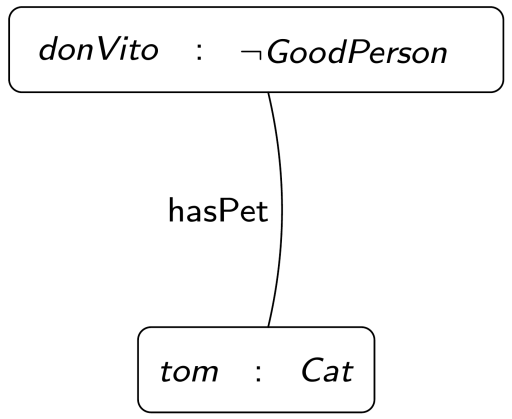
\includegraphics[width=0.5\linewidth]{img/tab1}
	\caption{Initial tableau}
	\label{fig:tab1}
\end{figure}

This means that if the opposite of the query is (artificially) added to the knowledge base as a new axiom, this ontology will contain at least two pieces of information one contradicting the other.

The tableau has one node for each individual: tom is labelled as cat, $donVito$ is labelled as not a good person (the negation of the query), and the edge between them is labelled as $hasPet$ because the individuals are connected by this property (Figure~\ref{fig:tab1}).

At this point, the graph of Figure~\ref{fig:tab1} is expanded using the axioms of the ontology to check the truth of the query and to build the justifications. Therefore, the tableau algorithm takes e.g. the axiom 3, ``cats are pets'', and adds to the node for tom also the label $pet$ since he is a cat. This new information is true and its justification is given directly by the set of axioms {1,3}: axiom 3 because since $tom$ is a $cat$ (axiom 1) he is also a $pet$. The same operation can be done for the edge (relationship) between tom and $donVito$, which can be labelled also as $hasAnimal$ because of axioms~2 and~6.

At this point, the calculus can deduce that $donVito$ belongs to the class \linebreak $\exists hasAnimal.Pet$ because $donVito$ is connected with $tom$, which is a $pet$ (axioms {1,3}), via property $hasAnimal$ (axioms {2,6}). Therefore, $donVito$’s node is labelled also as $\exists hasAnimal.Pet$ with a justification given by the union of the axioms associated with the used axioms, therefore its justification is given by the set of the involved axioms {1,2,3,6}. Then, the tableau graph is further expanded by adding the class $NatureLover$ to $donVito$’s node using axiom 4 and finally, by adding also the class $GoodPerson$ using label $NatureLover$ (axioms {1,2,3,4,6}) and axiom 5, creating as justification the set of axioms {1,2,3,4,5,6}.

The final graph is shown in Figure~\ref{fig:tab2}.
\begin{figure}
	\centering
	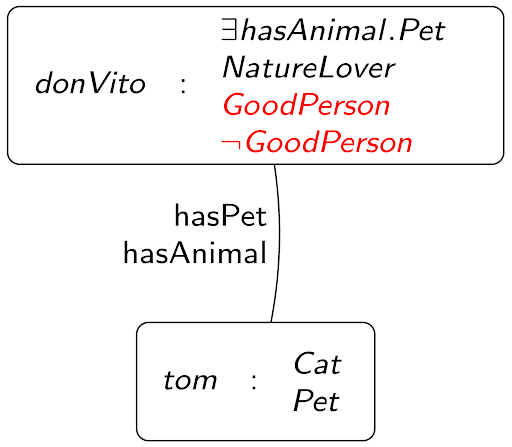
\includegraphics[width=0.5\linewidth]{img/tab2}
	\caption{Initial tableau}
	\label{fig:tab2}
\end{figure}
The expanded graph contains now a contradiction, i.e., $donVito$ is labelled as $GoodPerson$ and as not a $GoodPerson$ (i.e., $\neg GoodPerson$), therefore, by refutation, the query ``Is don Vito Corleone a good person?'' is true, with justification given by the axioms {1,2,3,4,5,6}, that are the axioms of the KB necessary to deduce this information.

From this example, it would be clear why the use of probabilistic information is useful. Indeed, don Vito Corleone is hardly classifiable as a good person. This is because not all people who are nature lovers are also good, and therefore, one could say that axiom 5 is true with probability 0.4. It would also be arguable that everyone who has animals is also a nature lover, making probabilistic also this axiom. For a formal description of how the probability of the query is computed see the Appendix~\ref{app:inf}.
\subsection{Possible Queries}
\label{queries}

TRILL can compute the probability or find an explanation of the following queries:
\begin{itemize}
  \item Concept membership queries.
  \item Property assertion queries.
  \item Subsumption queries.
  \item Unsatifiability of a concept.
  \item Inconsistency of the knowledge base.
\end{itemize}
All the input arguments must be atoms or ground terms.
Note that it is necessary to specify which algorithm, TRILL, TRILL$^P$ or TORNADO, has to be loaded for performing inference. This is done by using at the beginning of the input file the directive
\begin{verbatim}
:- trill.
\end{verbatim}
for loading TRILL,
\begin{verbatim}
:- trillp.
\end{verbatim}
for TRILL$^P$ or
\begin{verbatim}
:- tornado.
\end{verbatim}
for TORNADO.

\subsubsection{Probabilistic Queries}
TRILL can be queried for computing the probability of queries. A resulting 0 probaility means that the query is false w.r.t. the knowledge base, while a probability value 1 that the query is certainly true.

The probability of an individual to belong to a concept can be asked using TRILL with the predicate
\begin{verbatim}
prob_instanceOf(+Concept:term,+Individual:atom,-Prob:double)
\end{verbatim}
as in (\href{http://trill.lamping.unife.it/example/trill/peoplePets.pl}{\texttt{peoplePets.pl}})
\begin{verbatim}
?- prob_instanceOf(cat,'Tom',Prob).
\end{verbatim}

The probability of two individuals to be related by a role can be computed with
\begin{verbatim}
prob_property_value(+Prop:atom,+Individual1:atom,
                    +Individual2:atom,-Prob:double)
\end{verbatim}
as in (\href{http://trill.lamping.unife.it/example/trill/peoplePets.pl}{\texttt{peoplePets.pl}})
\begin{verbatim}
?- prob_property_value(has_animal,'Kevin','Tom',Prob).
\end{verbatim}

If you want to know the probability with which a class is a subclass of another you have to use
\begin{verbatim}
prob_sub_class(+Concept:term,+SupConcept:term,-Prob:double)
\end{verbatim}
as in (\href{http://trill.lamping.unife.it/example/trill/peoplePets.pl}{\texttt{peoplePets.pl}})
\begin{verbatim}
?- prob_sub_class(cat,pet,Prob).
\end{verbatim}

The probability of the unsatisfiability of a concept can be asked with the predicate
\begin{verbatim}
prob_unsat(+Concept:term,-Prob:double)
\end{verbatim}
as in (\href{http://trill.lamping.unife.it/example/trill/peoplePets.pl}{\texttt{peoplePets.pl}})
\begin{verbatim}
?- prob_unsat(intersectionOf([cat,complementOf(pet)]),P).
\end{verbatim}
This query for example corresponds with a subsumption query, which is represented as the intersection of the subclass and the complement of the superclass.

Finally, you can ask the probability of the inconsistency of the knowledge base with
\begin{verbatim}
prob_inconsistent_theory(-Prob:double)
\end{verbatim}


\subsubsection{Non Probabilistic Queries}
In TRILL you can also ask whether a query is true or false w.r.t. the knowledge base and in case of a succesful query an explanation can be returned as well. 
Query predicates in this case differs in the number of arguments, in the second case, when we want also an explanation, an extra argument is added to unify with the list of axioms
build to explain the query.

The query if an individual belongs to a concept can be used the predicates
\begin{verbatim}
instanceOf(+Concept:term,+Individual:atom)
instanceOf(+Concept:term,+Individual:atom,-Expl:list)
\end{verbatim}
as in (\href{http://trill.lamping.unife.it/example/trill/peoplePets.pl}{\texttt{peoplePets.pl}})
\begin{verbatim}
?- instanceOf(pet,'Tom').
?- instanceOf(pet,'Tom',Expl).
\end{verbatim}
In the first query the result is \verb|true| because Tom belongs to cat, in the second case TRILL returns the explanation 
\begin{verbatim}
[classAssertion(cat,'Tom'), subClassOf(cat,pet)]
\end{verbatim}


Similarly, to ask whether two individuals are related by a role you have to use the queries
\begin{verbatim}
property_value(+Prop:atom,+Individual1:atom,+Individual2:atom)
property_value(+Prop:atom,+Individual1:atom,
               +Individual2:atom,-Expl:list)
\end{verbatim}
as in (\href{http://trill.lamping.unife.it/example/trill/peoplePets.pl}{\texttt{peoplePets.pl}})
\begin{verbatim}
?- property_value(has_animal,'Kevin','Tom').
?- property_value(has_animal,'Kevin','Tom',Expl).
\end{verbatim}

If you want to know if a class is a subclass of another you have to use
\begin{verbatim}
sub_class(+Concept:term,+SupConcept:term)
sub_class(+Concept:term,+SupConcept:term,-Expl:list)
\end{verbatim}
as in (\href{http://trill.lamping.unife.it/example/trill/peoplePets.pl}{\texttt{peoplePets.pl}})
\begin{verbatim}
?- sub_class(cat,pet).
?- sub_class(cat,pet,Expl).
\end{verbatim}

The unsatisfiability of a concept can be asked with the predicate
\begin{verbatim}
unsat(+Concept:term)
unsat(+Concept:term,-Expl:list)
\end{verbatim}
as in (\href{http://trill.lamping.unife.it/example/trill/peoplePets.pl}{\texttt{peoplePets.pl}})
\begin{verbatim}
?- unsat(intersectionOf([cat,complementOf(pet)])).
?- unsat(intersectionOf([cat,complementOf(pet)]),Expl).
\end{verbatim}
In this case, the returned explanation is the same obtained by querying if cat is subclass of pet with the \verb|sub_class/3| predicate, i.e., \verb|[subClassOf(cat,pet)]|

Finally, you can ask about the inconsistency of the knowledge base with
\begin{verbatim}
inconsistent_theory
inconsistent_theory(-Expl:list)
\end{verbatim}

The predicate above returns explanations one at a time. To collect all the explanations with a single goal you can use the predicates:
\begin{verbatim}
all_instanceOf(+Concept:term,+Individual:atom,-Expl:list)
all_property_value(+Prop:atom,+Individual1:atom,
                        +Individual2:atom,-Expl:list)
all_sub_class(+Concept:term,+SupConcept:term,-Expl:list)
all_unsat(+Concept:term,-Expl:list)
all_inconsistent_theory(-Expl:list)
\end{verbatim}

\subsection{Query Options}
The behaviour of the queries can be fine tuned using the \emph{query options}. To use them you need to use the predicates:
\begin{verbatim}
instanceOf(+Concept:term,+Individual:atom,-Expl:list,-QueryOptions:list)
property_value(+Prop:atom,+Individual1:atom,
                        +Individual2:atom,-Expl:list,-QueryOptions:list)
sub_class(+Concept:term,+SupConcept:term,-Expl:list,-QueryOptions:list)
unsat(+Concept:term,-Expl:list,-QueryOptions:list)
inconsistent_theory(-Expl:list,-QueryOptions:list)
\end{verbatim}

Options can be:
\begin{itemize}
	\item \verb|assert_abox(Boolean)| if Boolean is set to true the list of ABoxes is asserted with the predicate \verb|final_abox/1|;
	\item \verb|return_prob(Prob)| if present the probability of the query is computed and unified with \verb|Prob|;
%	\item \verb|return_single_prob(Boolean)| must be used with \verb|return_prob(Prob)|. It forces TRILL to return the probability of each single explanation;
	\item \verb|max_expl(Value)| to limit the maximum number of explanations to find. \verb|Value| must be an integer. The predicate will return a list containing at most \verb|Value| different explanations;
	\item \verb|time_limit(Value)| to limit the time for the inference. The predicate will return the explanations found in the time allowed. \verb|Value| is the number of seconds allowed for the search of explanations .
\end{itemize}

For example, if you want to find the probability of the query $Q=kevin:PetOwner$ computed on at most 2 explanations allowing at most 1 second for the explanations search you can use the goal
\begin{verbatim}
instanceOf('natureLover','Kevin',Expl,
           [time_limit(1),return_prob(Prob),max_expl(2)]).
\end{verbatim}

\subsection{TRILL Useful Predicates}
There are other predicates defined in TRILL which helps manage and load the KB.
\begin{verbatim}
add_kb_prefix(++ShortPref:string,++LongPref:string)
add_kb_prefixes(++Prefixes:list)
\end{verbatim}
They register the alias for prefixes. The firs registers \verb|ShortPref| for the prefix \verb|LongPref|, while the second register all the alias prefixes contained in Prefixes. The input list must contain pairs alias=prefix, i.e., \verb|[('foo'='http://example.foo#')]|. In both cases, the empty string \verb|''| can be defined as alias. The predicates
\begin{verbatim}
remove_kb_prefix(++ShortPref:string,++LongPref:string)
remove_kb_prefix(++Name:string)
\end{verbatim}
remove from the registered aliases the one given in input. In particular, \verb|remove_kb_prefix/1| takes as input a string that can be an alias or a prefix and removes the pair containing the string from the registered aliases.

\begin{verbatim}
add_axiom(++Axiom:axiom)
add_axioms(++Axioms:list)
\end{verbatim}
These predicates add (all) the given axiom to the knowledge base. While, to remove axioms can be similarly used the predicates
\begin{verbatim}
remove_axiom(++Axiom:axiom)
remove_axioms(++Axioms:list)
\end{verbatim}
All the axioms must be defined following the TRILL syntax.

Finally, we can interrogate TRILL to return the loaded axioms with
\begin{verbatim}
axiom(?Axiom:axiom)
\end{verbatim}
This predicate searches in the loaded knowledge base axioms that unify with Axiom.

\subsection{Executing a Query with TRILL}
To run a query, you can simply load the Prolog file, for example \href{http://trill.lamping.unife.it/example/trill/peoplePets.pl}{\texttt{peoplePets.pl}}, as
\begin{verbatim}
?- [peoplePets].
\end{verbatim}
\noindent
The linked file contains axioms defined in both syntaxes accepted by TRILL, RDF/XML and Prolog Syntax, based on definition of \href{http://vangelisv.github.io/thea/}{Thea} library.
\href{http://trill.lamping.unife.it/example/trill/peoplePets.pl}{\texttt{peoplePets.pl}} is equivalent with the following KB
\begin{verbatim}
:- use_module(library(trill)).

:- trill.

:- add_kb_prefix('','http://cohse.semanticweb.org/ontologies/people#').

subClassOf(someValuesFrom('has_animal', 'pet'), 'natureLover').
subClassOf('cat', 'pet').
annotationAssertion('disponte:probability', 
        classAssertion('cat', 'Fluffy'), literal('0.4')).
annotationAssertion('disponte:probability', 
        classAssertion('cat', 'Tom'), literal('0.3')).
annotationAssertion('disponte:probability', 
        subClassOf('cat', 'pet'), literal('0.6')).
propertyAssertion('has_animal', 'Kevin', 'Fluffy').
propertyAssertion('has_animal', 'Kevin', 'Tom').
classAssertion('cat', 'Fluffy').
classAssertion('cat', 'Tom').
\end{verbatim}
\noindent


You can also load an RDF/XML file using the predicate \verb|load_owl_kb(<filename>).| in the following way:
\begin{itemize}
	\item load TRILL library\\
	\verb|use_module(library(trill)).|
	\item initialize the algorithm you want to perform inference\\
	\verb|init_trill(<algorithm_name>).|\\
	For example, if you want to use TRILL$^P$ you should run \verb|init_trill(trillp).|
	\item load the KB\\
	\verb|load_owl_kb(<filename>).|\\
	For example, \verb|load_owl_kb('./examples/biopaxLevel3_rdf.owl').|
\end{itemize}
\noindent
Now the KB is loaded and the queries can be executed in the usual way.

\subsection{Files}
The \texttt{pack/trill/prolog/examples} folder in SWI-Prolog home contains some example programs.
The \texttt{pack/trill/doc} folder in SWI-Prolog home contains this manual in latex, html and pdf.


\section{License}
\label{license}



TRILL follows the Artistic License 2.0 that you can find in TRILL root folder. The copyright is by Riccardo Zese.
\vspace{3mm}

The library \href{http://vangelisv.github.io/thea/}{Thea} at the basis of the translation module is available under the \href{http://www.gnu.org/copyleft/gpl.html}{GNU/GPL license}.

The library \href{http://vlsi.colorado.edu/\string ~fabio/}{CUDD} for manipulating BDDs has the following license:

\vspace{3mm}

Copyright (c) 1995-2004, Regents of the University of Colorado

All rights reserved.

Redistribution and use in source and binary forms, with or without
modification, are permitted provided that the following conditions
are met:

\begin{itemize}
\item
Redistributions of source code must retain the above copyright
notice, this list of conditions and the following disclaimer.
\item
Redistributions in binary form must reproduce the above copyright
notice, this list of conditions and the following disclaimer in the
documentation and/or other materials provided with the distribution.
\item
Neither the name of the University of Colorado nor the names of its
contributors may be used to endorse or promote products derived from
this software without specific prior written permission.
\end{itemize}
THIS SOFTWARE IS PROVIDED BY THE COPYRIGHT HOLDERS AND CONTRIBUTORS
"AS IS" AND ANY EXPRESS OR IMPLIED WARRAN\-TIES, INCLUDING, BUT NOT
LIMITED TO, THE IMPLIED WARRANTIES OF MERCHANTABILITY AND FITNESS
FOR A PARTICULAR PURPOSE ARE DISCLAIMED. IN NO EVENT SHALL THE
COPYRIGHT OWNER OR CONTRIBUTORS BE LIABLE FOR ANY DIRECT, INDIRECT,
INCIDENTAL, SPECIAL, EXEMPLARY, OR CONSEQUENTIAL DAMAGES (INCLUDING,
BUT NOT LIMITED TO, PROCUREMENT OF SUBSTITUTE GOODS OR SERVICES;
LOSS OF USE, DATA, OR PROFITS; OR BUSINESS INTERRUPTION) HOWEVER
CAU-SED
\\ AND ON ANY THEORY OF LIABILITY, WHETHER IN CONTRACT, STRICT
LIABILITY, OR TORT (INCLUDING NEGLIGENCE OR OTHERWISE) ARISING IN
ANY WAY OUT OF THE USE OF THIS SOFTWARE, EVEN IF ADVISED OF THE
POSSIBILITY OF SUCH DAMAGE.


\bibliographystyle{plain}
\bibliography{bib}

\end{document}
